% Layout assembly, 2026-10-01. Previous tables and prose slots are preserved in
% draft_archive/2026-10-01_before_asset_mockups/5_results.tex.
% No new experimental measurements are reported by this draft.
\section{Experiments}
\label{sec:exp}

\noindent\textbf{Layout draft.}
The following figures and tables specify the planned comparisons.
AI-generated scenes and synthetic curves are explicitly marked and are not
experimental evidence. The HumanTech convergence figure contains historical
results and will be replaced with measurements from the final implementation.
All quantitative table entries are left blank.

\subsection{Setup}
\label{ssec:setup}

\noindent\textbf{Datasets and metrics.}
The candidate evaluation set comprises the public RGB--IMU datasets RPNG and
UTMM, and sequences captured with Aria glasses.
We reserve PSNR, SSIM, and LPIPS columns for images excluded from training,
alongside tracking error, final Gaussian count, and peak memory.
The complete candidate sequence list appears in the supplementary tables;
the final common evaluation subset and split remain to be locked.

\noindent\textbf{Comparison protocols.}
We separate matched training-render budgets from matched elapsed-time budgets.
For equal-time comparisons, tracking runs concurrently and the same sensor
timestamps determine frame arrivals. The two time allowances are
1$\times$ and 1.5$\times$ the sensor-record duration, with no optimization
after the last input frame.
Candidate systems are grouped by their actual input modality. Monocular
RGB methods and RGB--IMU methods must not be interpreted as identical-input
comparisons. Any method requiring sensor depth is excluded from this protocol;
the conditional MM3DGS-SLAM row requires a verified monocular RGB--IMU setup.

\subsection{Rendering Quality and Convergence}
\label{ssec:main}

Table~\ref{tab:rendering_comparison} reserves dataset-mean comparisons;
Table~\ref{tab:scene} gives the corresponding sequence-level template.
Figure~\ref{fig:photometric_convergence} reuses the HumanTech convergence
layout, while Figure~\ref{fig:new_region} specifies how appearance and geometry
will be evaluated after a region first becomes observable.
Figure~\ref{fig:rgb_comparison} reserves matched held-out views and common
enlarged regions for qualitative comparison.

\input{tab/t1_main_draft}
\begin{figure}[tbp]
  \centering
  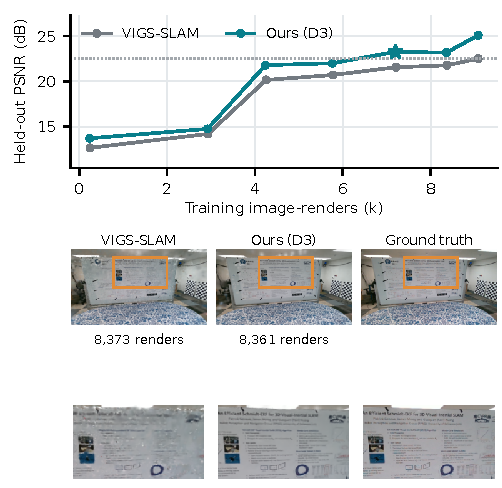
\includegraphics[width=\linewidth]{figs/draft/f3.pdf}
  \caption{Measured photometric convergence on RPNG \texttt{table\_06} at 40 training renders/KF. The starred checkpoint first reaches the baseline's highest observed PSNR with 1,879 fewer training renders on the sampled grid. Below: held-out renderings and shared GT-selected enlargements at the same streaming prefix; actual render counts are shown. The curve uses a fixed uniform held-out subset. D3 proxy renders are additional work.}
  \label{fig:photometric_convergence}
\end{figure}

\begin{figure}[tbp]
  \centering
  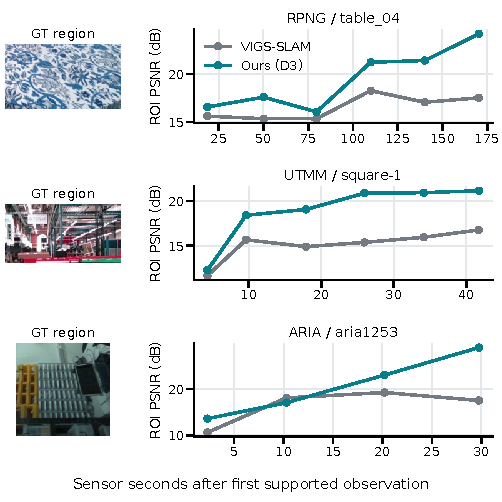
\includegraphics[width=\linewidth]{figs/draft/f4.pdf}
  \caption{Measured refinement of matched held-out RGB regions. Points show PNG ROI PSNR at actual map checkpoints; the horizontal axis is sensor time after the first feature-supported observation, not wall-clock time. GT structure selects examples from all 20 scenes. D3 adds proxy renders.}
  \label{fig:new_region}
\end{figure}

\begin{figure}[tbp]
  \centering
  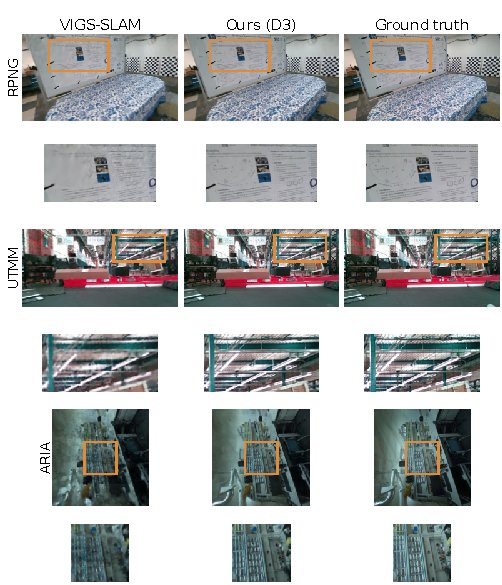
\includegraphics[width=\linewidth]{figs/draft/f5.pdf}
  \caption{Actual final held-out renderings at 40 training renders/KF. Columns: VIGS-SLAM, ours and GT. Rows: RPNG \texttt{table\_06}; UTMM \texttt{square-1}; ARIA \texttt{aria1253}. Shared enlarged regions are selected from GT structure. All 20 candidates were evaluated before selection. D3 adds proxy renders.}
  \label{fig:rgb_comparison}
\end{figure}


\subsection{Equal-Time Online Comparison}
\label{ssec:time_results}

Table~\ref{tab:time_comparison} reserves quality and resource measurements
under both time allowances. Figure~\ref{fig:equal_time} aligns quality curves
with completed training work at common elapsed-time checkpoints.
Figure~\ref{fig:tracking_capacity} relates tracking load and keyframe arrivals
to achieved mapping work per keyframe; it does not estimate a hardware limit
from the synthetic example.
Table~\ref{tab:baseline_peak} compares the work needed to first reach each
sequence's highest observed baseline PSNR. An unreached target will be marked
NR rather than assigned a fabricated crossing cost.

\input{tab/t2_main_draft}
\begin{figure}[tbp]
  \centering
  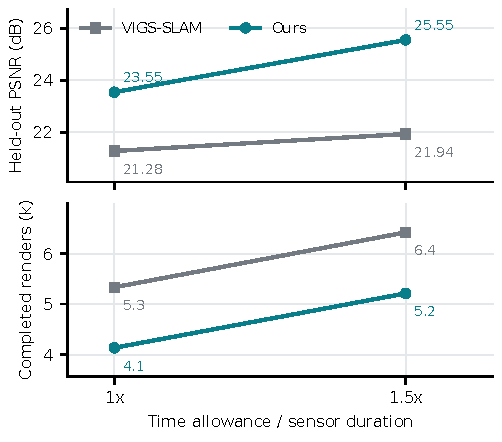
\includegraphics[width=\linewidth]{figs/draft/f11.pdf}
  \caption{Measured final quality and completed training renders with concurrent tracking. Each point averages 2 completed sequence pairs from separate runs at 1$\times$/1.5$\times$ time allowances. These are budget-response endpoints. Both systems use the same dataset Tracking configuration; tracking can finish after the mapper deadline.}
  \label{fig:equal_time}
\end{figure}

\begin{figure}[tbp]
  \centering
  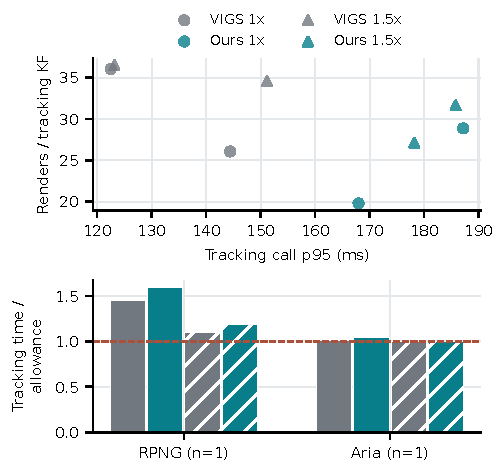
\includegraphics[width=\linewidth]{figs/draft/f12.pdf}
  \caption{Shared-tracker measurements on 2 paired sequences at 1$\times$/1.5$\times$ allowances. Top: observed tracking-call p95 versus committed training renders per final tracking KF, including KFs not admitted to mapping. Bottom: tracking completion time divided by allowance (dataset scene means); values above one exceed the mapper deadline. The mapper cap is 40 renders/admission. These measurements do not establish a causal tracking-cost effect or a hardware limit.}
  \label{fig:tracking_capacity}
\end{figure}

\input{tab/t6_peak_draft}

\subsection{Geometry}
\label{ssec:geometry_results}

Table~\ref{tab:geometry} reserves free-space and surface-quality measurements
alongside held-out rendering quality.
Figures~\ref{fig:carve} and~\ref{fig:geometry_convergence} specify complementary
solid-ellipsoid cutaways and geometry-convergence curves. Reference geometry,
region masks, and evaluation thresholds must be fixed before populating them.

\input{tab/t3_geometry_draft}
\begin{figure}[tbp]
  \centering
  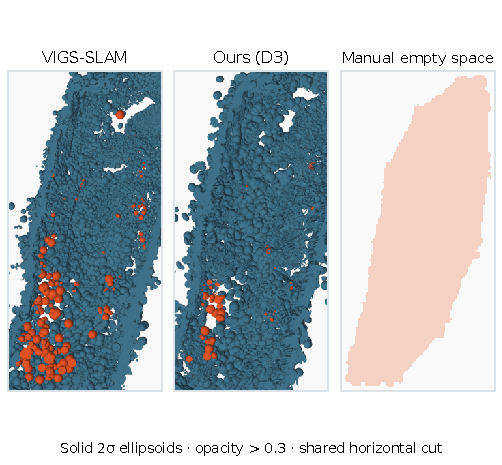
\includegraphics[width=\linewidth]{figs/draft/f6.pdf}
  \caption{Actual Aria1253 maps at 40 training renders/KF as solid $2\sigma$ covariance ellipsoids. The view, horizontal cut and opacity cutoff ($>0.3$) are shared. Orange centers lie in the independent manual empty-space mask; blue centers lie outside. Right: the annotation, not a surface reference. This compares complete systems; D3 adds proxy renders.}
  \label{fig:carve}
\end{figure}

\begin{figure}[tbp]
  \centering
  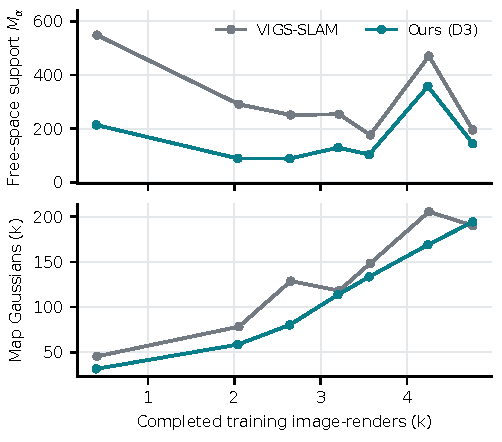
\includegraphics[width=\linewidth]{figs/draft/f7.pdf}
  \caption{Independent free-space diagnostics on Aria1253. Top: opacity-weighted covariance support in a fixed manual region within shared first-checkpoint camera frusta (71.8\% of the annotation). Bottom: map size. Markers are actual checkpoints; map growth can increase the error. Frustum inclusion does not establish surface visibility or completeness. This compares complete systems; D3 adds proxy renders.}
  \label{fig:geometry_convergence}
\end{figure}


\subsection{Ablations}
\label{ssec:abl}

Table~\ref{tab:order} retains the original replay experiment's
15/30/60-update comparison between random reshuffling and the entropy-regularized
sampler. Figure~\ref{fig:sampling_convergence} reserves the corresponding
convergence curves. Results from the original replay sampler and the current
online ERVS implementation will be identified separately.
Table~\ref{tab:abl} compares keyframe-only supervision with additional
between-keyframe images in one shared engine and under the same budget.
These tables contain no historical or synthetic scores.

\input{tab/t4_sampling_draft}
\begin{figure}[tbp]
  \centering
  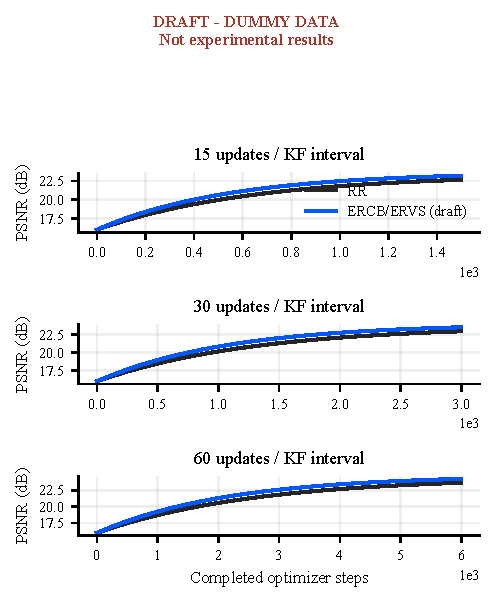
\includegraphics[width=\linewidth]{figs/draft/f9.pdf}
  \caption{\textbf{Dummy data.} Sampling convergence at 15/30/60 updates per keyframe interval. Sampler labels await reconciliation with the measured replay implementation.}
  \label{fig:sampling_convergence}
\end{figure}

\input{tab/t5_dense_draft}
\clearpage
